\documentclass{scrartcl}
\usepackage[utf8]{inputenc}
\usepackage{tikz}
\begin{document}
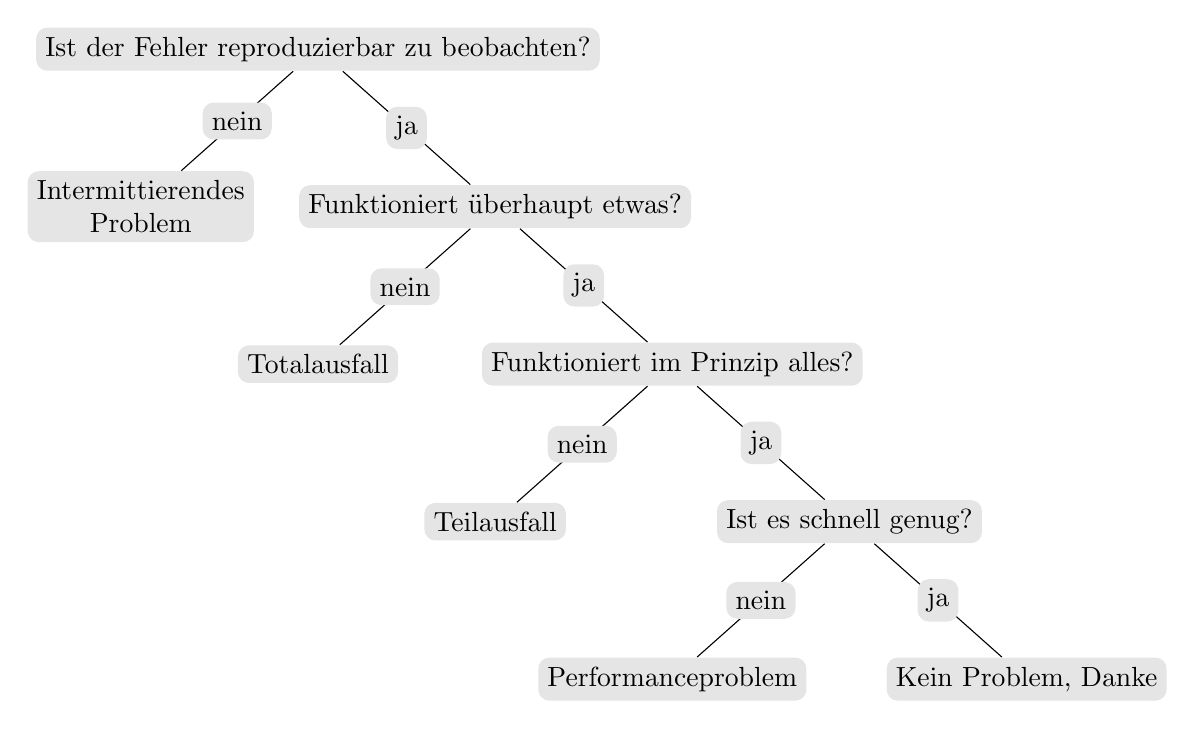
\begin{tikzpicture}
[every node/.style={fill=black!10,rounded corners,align=center},
grow=south, level distance=2cm,
level 1/.style={sibling distance=4.5cm},
level 2/.style={sibling distance=4.5cm},
]

\node{Ist der Fehler reproduzierbar zu beobachten?}
  child{node{Intermittierendes\\Problem}
  edge from parent node{nein}}
  child{node{Funktioniert überhaupt etwas?}
    child{node{Totalausfall} edge from parent node{nein}}
    child{node{Funktioniert im Prinzip alles?}
      child{node{Teilausfall} edge from parent node{nein}}
      child{node{Ist es schnell genug?}
        child{node{Performanceproblem} edge from parent node{nein}}
        child{node{Kein Problem, Danke}
	edge from parent node{ja}}
      edge from parent node{ja}}
    edge from parent node{ja}}
  edge from parent node{ja}};
\end{tikzpicture}
\end{document}
